%
% PROJECT: <ETD> Electronic Thesis and Dissertation Initiative
%   TITLE: LaTeX report template for ETDs in LaTeX
%  AUTHOR: Neill Kipp, nkipp@vt.edu
%     URL: http://etd.vt.edu/latex/
% SAVE AS: etd.tex
% REVISED: September 6, 1997 [GMc 8/30/10]
% 

% Instructions: Remove the data from this document and replace it with your own,
% keeping the style and formatting information intact.  More instructions
% appear on the Web site listed above.

\documentclass[12pt]{report}
% \documentclass[12pt,dvips]{report} %% TODO CHANGED THIS .. removed dvips .. printer friendly


\setlength{\textwidth}{6.5in}
\setlength{\textheight}{8.5in}
\setlength{\evensidemargin}{0in}
\setlength{\oddsidemargin}{0in}
\setlength{\topmargin}{0in}

\setlength{\parindent}{0pt}
\setlength{\parskip}{0.1in}

%\setcounter{secnumdepth}{3}
%\setcounter{tocdepth}{3}

% Uncomment for double-spaced document.
\renewcommand{\baselinestretch}{1.3}
\newcommand{\des}{\textit{Discrete Event Simulator}}
\usepackage{graphicx}
\graphicspath{ {images/} }
%\graphicspath{ {/root/thesis/images/} }
\usepackage{url, listings, color}
\usepackage{etoolbox}
\usepackage [ruled,vlined,algo2e]{algorithm2e}
\newbool{toShowBibliography} % var to show bibliography


\usepackage{titlesec}
\usepackage{hyperref}

\titleclass{\subsubsubsection}{straight}[\subsection]

\newcounter{subsubsubsection}
\renewcommand\thesubsubsubsection{\thesubsubsection.\arabic{subsubsubsection}}
\renewcommand\theparagraph{\thesubsubsubsection.\arabic{paragraph}} % optional; useful if paragraphs are to be numbered

\titleformat{\subsubsubsection}
  {\normalfont\normalsize\bfseries}{\thesubsubsubsection}{1em}{}
\titlespacing*{\subsubsubsection}
{0pt}{3.25ex plus 1ex minus .2ex}{1.5ex plus .2ex}

\makeatletter
\renewcommand\paragraph{\@startsection{paragraph}{5}{\z@}%
  {3.25ex \@plus1ex \@minus.2ex}%
  {-1em}%
  {\normalfont\normalsize\bfseries}}
\renewcommand\subparagraph{\@startsection{subparagraph}{6}{\parindent}%
  {3.25ex \@plus1ex \@minus .2ex}%
  {-1em}%
  {\normalfont\normalsize\bfseries}}
\def\toclevel@subsubsubsection{4}
\def\toclevel@paragraph{5}
\def\toclevel@paragraph{6}
\def\l@subsubsubsection{\@dottedtocline{4}{7em}{4em}}
\def\l@paragraph{\@dottedtocline{5}{10em}{5em}}
\def\l@subparagraph{\@dottedtocline{6}{14em}{6em}}
\makeatother
\setcounter{secnumdepth}{4}
\setcounter{tocdepth}{4}


\begin{document}

\thispagestyle{empty}
\pagenumbering{roman}
\begin{center}

% TITLE
{\Large 
Device Driver isolation using virtual machines
}

\vfill

Sushrut Shirole

\vfill

Thesis submitted to the Faculty of the \\
Virginia Polytechnic Institute and State University \\
in partial fulfillment of the requirements for the degree of

\vfill

Master of Science \\
in \\
Computer Science \& Applications

\vfill

Dr. Godmar Back, Chair \\
Dr. Keith Bisset \\
Dr. Kirk Cameron\\


\vfill

Dec 12, 2013 \\
Blacksburg, Virginia

\vfill

Keywords: Device driver, Virtual machines, domain,  
\\
Copyright 2013, Sushrut Shirole

\end{center}

\pagebreak

\thispagestyle{empty}
\begin{center}

{\large 
Device driver isolation using virtual machines.
}

\vfill

Sushrut Shirole

\vfill

(ABSTRACT)
\end{center}

In majority of today's operating system architectures, kernel is tightly coupled with the device drivers. In such cases, failure in critical components can lead to system failure.
A malicious or faulty device driver can make the system unstable, thereby reducing the robustness. Unlike user processes, a simple restart of the device driver is not possible. In such circumstances a complete system reboot is necessary for complete recovery. In a virtualized environment or infrastructure where multiple operating systems execute over a common hardware platform, cannot afford to reboot the entire hardware due to a malfunctioning of a third party device driver. 
 
The solution we implement exploits the virtualization to isolate the device drivers from the kernel. In this implementation, a device driver serves the user process by running in a separate virtual machine and hence is isolated from kernel. This proposed solution increases the robustness of the system, benefiting all critical systems.
 
To support the proposed solution, we implemented a prototype based on linux kernel and Xen hypervisor. In this prototype we create an independent device driver domain for Block device driver. Our prototype demonstrate that a block device driver can be run in a separate domain. 
 
We isolate device drivers from the kernel with two different approaches and compare both the results. In first approach, we implement the device driver isolation using an interrupt-based inter-domain signaling facility provided by xen hypervisor called event channels. In second approach, we implement the solution, using spinning threads. In second approach user application puts the request in request queue asynchronously and independent driver domain spins over the request queue to check if a new request is available. Event channel is an interrupt-based inter-domain mechanism and it involves immediate context switch, however, spinning doesn't involve immediate context switch and hence can give different results than event channel mechanism. 


\vfill

% GRANT INFORMATION

\pagebreak

% Dedication and Acknowledgments are both optional
% \chapter*{Dedication}

\chapter*{Acknowledgments}
% TODO edit
Firstly, I would like to thank my advisor, Dr. Godmar Back. Under his guidance, I have acquired knowledge across a broad spectrum of computer science topics. I greatly appreciate the time he has dedicated toward our weekly meetings. I would like to thank Dr. Keith Bisset and Dr. Madhav Marathe for supporting me throughout my masters. I would like to thank Dr. Cameron for his role as a committee member and offering Computer Architecture course, which helped me learn the fundamentals.
\\
Last but not least, I am grateful to my family for their exceptional love, support and encouragement.  
% ref
\ifbool{toShowBibliography}{\bibliography{references}}{}

\tableofcontents
\pagebreak

\listoffigures
\pagebreak

\listoftables
\pagebreak

\pagenumbering{arabic}
\pagestyle{myheadings}

%%%%%%%%%%%%%%%%%%%%%%%%%%%%%%%%

\chapter{Introduction} 
\markright{Sushrut Shirole \hfill Chapter 1. Introduction \hfill}

% TODO edit

A system is judged by the quality of services it offer and its ability to function reliably. Even though reliability of operating system has been studied for several decades, it remains a major concern even today. Characteristics of operating system which makes them unstable and insecure are size and complexity. If we consider Linux kernel; it has over 15 million lines of code. One of the software reliability study shows that a code contains 6 to 16 bugs per 1000 lines of executable code\cite{Basili:1984:SEC:69605.2085}\cite{Tanenbaum06canwe}. Some other studies even says 2 to 75 bugs per 1000 lines of code \cite{Ostrand:2002:DFL:566172.566181}. Using a minimum estimate of 6 bugs per 1000 lines, the Linux kernel has around 90,000 bugs. Also one of the study shows that the device drivers have error rate 3 to 7 times higher than ordinary code\cite{Chou:2001:ESO:502034.502042}. So considering the fact that 70\% of the operating system consists of device drivers, our calculation of 90000 bugs can be an understatement\cite{Chou:2001:ESO:502034.502042}. To make a system reliable, finding all these bugs and fixing them is definitely not a feasible option considering the fact that bug fixes introduces new lines of code and hence new bugs.

\pagebreak

\section {Problem Statement}

Large size of system makes it impossible for one person to understand the code. At the same time complexity and tightly coupled device drivers and linux kernel makes it difficult to isolate a fault in a device driver. Difficulty in isolating faults in a device driver makes system unreliable and less robust, and hence the problem we try to solve here is of tightly coupled operating system. 

Monolithic kernel components doesn’t have the kind of isolation user level applications has. In a monolithic kernel, one of the millions lines of the kernel can overwrite kernel data structure used by an unrelated component and crash the system. This threat can be reduced by executing each device driver in an isolated environment from kernel. But a device driver is dependent upon many kernel components like memory management, scheduler etc., hence it is difficult to isolated device driver from kernel and execute it separately.

\pagebreak
  
\section {Proposed Solution} 
Unlike user applications, modern operating system kernel contains couple of hundred or thousand procedures linked together as a single program\cite{Tanenbaum06canwe}. Any one of the millions lines of the kernel can overwrite/corrupt kernel data structure.

In modern operating systems "Memory protection" is a way to control memory access rights. Memory protection prevents a process from accessing memory that has not been allocated to it, preventing a line of code within a process affecting other processes, or the operating system\cite{Denning:1970:VM:356571.356573}\cite{Galvin}. Unlike user applications, kernel has hundreds of procedure linked together, which makes it difficult to prevent an access to kernel data structure with memory protection.

The idea is to run a special program called a hypervisor. Hypervisor is capable of running multiple operating systems at a same time called as a virtual machine\cite{Goldberg:1973:AVM:800122.803950}. Hypervisor is commonly used to allow running of different operating systems such as Linux, Oracle, and Windows at same time, or is used to exploit the hardware. The use of virtual machines has a well-deserved reputation for extremely good fault isolation. Since none of the virtual machines even know about the other ones, malfunctioning of one virtual machine cannot spread to other\cite{LeVasseur04UnmodifiedDriverReuse}.

We propose an infrastructure which exploits the virtualization to isolate such linked procedures. In a virtualized environment, each virtual machine has an allocated memory, and because of memory protection mechanism, one virtual machine can not affect the memory of any other virtual machine. 

Exploiting this property we run a kernel and device driver in a new virtual machine, whereas user application and a kernel runs in separate virtual machine, making it impossible to corrupt kernel data structure by a device driver running in another virtual machine. Isolation of a device driver and a kernel can be achieved by running device driver in separate virtual machine than virtual machine which is running user application. Our solution here adapts the concept, protection of faults in an operating system\cite{LeVasseur04UnmodifiedDriverReuse}.

\pagebreak

\section{Core Contributions}

Technical core contributions of this report with respect to operating system design can be divided into two parts. 
\begin{enumerate}
\item Device driver isolation implementation 
\item Performance comparison of spinning and event channel.
\end{enumerate}

These contributions are listed below. 

\subsection{Device driver isolation}

An approach based on virtualization to decouple device driver from linux kernel, and partition existing kernel into application domain, and isolated device driver domain. Application domain would serve system calls related to core linux kernel functionality, whereas isolated device driver would serve system calls related to corresponding device driver.

\subsection{Performance comparison}

We implement request and response availability notification with mechanism provided by xen, which follows interrupt based model. We implement same part with spinning of threads to avoid context switch and compare the performance of isolated device driver.

We aim to find if there is any perfomance degradation in system because of context switch.

\pagebreak
\section {Organization}

This section gives the organization and roadmap of the thesis.

\begin{enumerate}
\item Chapter 2 gives the background on memory protection, virtualization, Xen Hypervisor, inter-domain communication, processes and threads. 
\item Chapter 3 gives the introduction to design of the system to isolate device driver. 
\item Chapter 4 discusses the detailed design and implementation to isolate device driver. 
\item Chapter 5 evaluate the performance of Independent device driver with different designs. 
\item Chapter 6 reviews related work in the area of kernel fault tolerance. 
\item Chapter 7 concludes the report and lists down the topics where this work can be extended.
\end{enumerate}

% ref
\ifbool{toShowBibliography}{\bibliography{references}}{}


\chapter{Background}  
\markright{Sushrut Shirole \hfill Chapter 2. Background \hfill}


\section{Memory protection}

\subsection{User space}

\subsection{kernel space}

\section{Virtualization}

\subsection{Hypervisor}

\subsection{Xen Hypervisor}

\subsubsection{Hypercalls and events}

\subsubsection{Data Transfer: I/O Rings}

\section{Processes and threads}

\subsection{Processes}

\subsection{Threads}

\subsection{Context Switch}

\subsection{Spinlocks and spinning}

\ifbool{toShowBibliography}{\bibliography{references}}{}


% System Overview/Architecture
\chapter{System Introduction}
\markright{Sushrut Shirole \hfill Chapter 3. System Introduction \hfill}

\section{Design Goal}\label{sec:goals}
The goal of the isolated driver domains is to provide strong isolation between a device driver and a monolithic kernel and at the same time to avoid modifications to the device driver code. The goal of the thesis is to reduce the performance penalty due to the communication between the domains. 

\subsection*{Performance Improvement}
The IDDR system is a re-implementation of isolated driver domains proposed by Fraser et. al. Even though IDDR system provides better robustness for the operating system, it suffers from performance overheads. The main reasons for the lower performance are the data copying overhead and the inter-domain communication overhead. 

\paragraph{Copying Overhead: } For write operation, a Linux system copies data from user space to kernel space and then from kernel space to the physical device. However, isolated driver domains system copies data from guest OS user space to guest OS kernel space, it then copies it to shared memory segment and from shared memory segment to the physical device. The extra copying of data in to the shared memory segment lowers the performance of the system. 

\paragraph{Communication Channel Overhead: } The application domain and the driver domain sends virtual interrupts when requests and responses are shared between both the domains. These virtual interrupts cause rescheduling of a domain in order to deliver the interrupts. Rescheduling of a domain can cause a context switch at an hypervisor level which adds an overhead to the system performance. Our goal is to reduce the overhead during communication between the driver domain and the application domain.

\section{Isolated Device Driver Properties}
\label{sec:properties}
This section covers the properties of the isolated driver domains. As we explore the opportunities to improve the performance of the isolated driver domains, it is necessary that these properties are not compromised.

\subsection*{Strong Isolation}
One of the main properties of the IDDR system is strong isolation. The isolated driver domains adds an extra layer of isolation in the design which provides fault isolation between the kernel and the device driver. It ensures that a bug within a device driver does not affect other kernel components.

\subsection*{Compatibility and Transparency} 
The extension of existing OS structures usually results in a large number of broken applications. Usually such extensions change the APIs visible to applications and breaks compatibility with the existing applications. The isolated driver domains does not change APIs visible to applications and device driver code and hence existing device drivers and applications are compatible with the new architecture.

\section{System Overview}\label{overview}

Figure~\ref{fig:monolithic} presents the architectural overview of the modern operating system with a monolithic kernel and Figure~\ref{fig:base IDDR system overview} presents the architectural overview of the IDDR system.
\\[3mm]
\begin{figure}[!ht]
\centering
\includegraphics[scale=.5]{OSoverview}
\caption{Architectural overview of a modern OS}
\label{fig:monolithic}
\end{figure}

\begin{figure}[!ht]
\centering
\includegraphics[scale=.5]{baseIDDRsystemoverview}
\caption{Architectural overview of the interrupt based IDDR system}
\label{fig:base IDDR system overview}
\end{figure}
The Figure~\ref{fig:base IDDR system overview} shows that IDDR system partitions an existing kernel into multiple independent components. User applications and the Linux kernel run in a domain called the \textit{application domain}. A device driver, which needs to be isolated from a kernel, executes in the separate domain called the \textit{driver domain}. Multiple domains run on the same hardware with the help of a VMM. User applications or kernel components access the hardware through the driver domain.
\\[3mm]
The goal of the IDDR system is to provide isolation between the device driver and the kernel. However, a device driver depends on kernel component such as a scheduler. Hence we run the device driver with an instance of a kernel and introduce a VMM into the design to run multiple kernels on a common hardware. 

\section{System Components}\label{components}
The section describes the 3 main components of the design - frontend driver, backend driver, and communication module.
\begin{figure}[!ht]
\centering
\includegraphics[scale=.5]{IDDRcomponents}
\caption{System Components}
\label{fig:Design Evo1}
\end{figure}

\subsection{Frontend Driver}
\label{subsec:frontend}
The IDDR system runs a piece of a code called the \textit{frontend driver} in an application domain. The \textit{frontend driver} acts as a substitute for the actual device driver. The main purpose of the \textit{frontend driver} is to accept requests from user applications, process the requests, enqueue the requests for the driver domain and notify the driver domain. The \textit{frontend driver} reads and processes the responses received from the driver domain and ends corresponding requests.

In a Linux system, user applications send requests to the actual device driver running in the same domain. However, in the IDDR system the actual device driver runs in a separate domain and the frontend driver helps user applications to forward requests to this actual device driver. Without the frontend device driver, we would have had to change existing applications in order to send requests to the actual device driver running in the driver domain. Hence, with introduction of the frontend driver we achieve the transperency goal.

\subsection{Backend Driver}
\label{subsec:backend}
The IDDR system runs a piece of a code called the \textit{backend driver} runs in the driver domain. The responsibility of the \textit{backend driver} is to accept requests from the application domain and forward them to the actual device driver. The \textit{backend driver} sends the responses and notifies the application domain after receiving the responses from the device driver.

In a Linux system, the actual device driver sends responses back to user applications running in the same domain. However, in the IDDR system, the backend driver sends responses to the frontend driver. Without the backend device driver, we would have had to change existing device drivers in order to send responses to user applications running in the application domain. Hence, with introduction of the backend driver we achieve the compatibility goal.

\begin{figure}[!ht]
    \centering
    \begin{subfigure}[b]{0.45\textwidth}
	\includegraphics[scale=.25]{component1}
	\caption{Conceptual design of the driver domain}
	\label{fig:conept}
    \end{subfigure}
	\hfill
    \begin{subfigure}[b]{0.45\textwidth}
	\includegraphics[scale=.25]{component2}
	\caption{Backend and frontend driver}
	\label{fig:backendfrontend}
    \end{subfigure}
    \caption{Role of the frontend and the backend drivers}\label{fig:fault tolerence}
\end{figure}

\subsection{Communication Module}
\label{sub:communicationmodule}
The communication module provides a communication channel between the \textit{frontend driver} and the \textit{backend driver}. The communication channel is logically divided into three parts. The responsibility of the communication module is to
\begin{enumerate} 
\item share the requests and responses between the driver domain and the application domain.
\item share the data of read/write requests/responses.
\item notify the domain upon the occurrence of a particular event. 
\end{enumerate}

Figure~\ref{fig:communication} provides the overview of the communication model. 
\begin{figure}[!ht]
\centering
\includegraphics[scale=.5]{communicationmodule}
\caption{Communication Module}
\label{fig:communication}
\end{figure}

\section{System Design}\label{design}

The following section describes the design of interrupt based IDDR system and spinning based IDDR system. 

\subsection{Communication Module}

\paragraph{Interrupt based IDDR System:}
\label{par:base IDDR communication}
In interrupt based IDDR system, the frontend driver submits requests to the communication module. The communication module copies data of the write requests in a shared memory. The communication module is responsible for the allocation and de-allocation of the shared memory page. Once a sufficient number of requests is submitted by the frontend driver, the communication channel shares the requests with the backend driver. It notifies the backend driver that requests are available in a shared request queue.

\paragraph{Spinning Based IDDR System:}
\label{par:spin IDDR communication}
In the interrupt based IDDR system, by default a software interrupt is sent to the domain as a notification. Each such software interrupt causes the hypervisor to schedule the driver domain. Similarly, software interrupts which notify the availability of responses, causes the hypervisor to schedule the application domain. The scheduling of the driver domain and the application domain might result in a context switch. 

In order to avoid these context switches, we run an intermediate thread in the frontend driver and an intermediate thread in the backend driver. Both threads spin for the availability of requests and responses in the shared queue. The intermediate threads delegate the responsibility of the notifications from the frontend driver and backend driver to the communication module. 

\subsection{Frontend Driver}
\paragraph{Interrupt based IDDR System Design:}
In the IDDR system, the frontend driver provides an interface to accept requests from a user application on behalf of the device driver. As explained in Section~\ref{subsec:request queue}, each block device driver has a separate request queue to accept requests from a user application. Similar to block device drivers, the frontend driver also creates an individual request queue for a device to accept requests from user applications. The frontend driver flushes the requests to the communication channel. The frontend driver receives a software interrupt upon the availability of responses in the shared queue. The frontend driver handles the software interrupt by reading data from the shared memory in case of read operation and sends a completion notification to a user application. Otherwise it sends a completion notification to a user application.

\paragraph{IDDR System Design:}
As explained in Section~\ref{par:spin IDDR communication}, we introduce an intermediate thread to read responses from the shared queue. The intermediate thread spins for responses. Upon availability of a response, the thread reads the response and sends a complition notification to a user application. If the corresponding request is a read request, then the thread reads the shared data too.

\begin{figure}[!ht]
\centering
\includegraphics[scale=.5]{IDDRdesign}
\caption{Spinning based IDDR system}
\label{fig:new IDDR system}
\end{figure}

% \section{fault tolerance}
% Figure~\ref{fig:driver crash} and Figure~\ref{fig:high avail} explains the effects of a malicious activity occurring in the device driver isolated from the Linux kernel. When a device driver running in a driver domain hits a bug, it crashes the kernel of the driver domain and hence the driver domain itself. In addition, applications expecting a response from the driver domain might hang or crash waiting for the response. But due to the address space separation of the application domain and the driver domain, the application domain will remain intact.   
% \begin{figure}[!ht]
%     \centering
%     \begin{subfigure}[b]{0.45\textwidth}
% 	\includegraphics[scale=.25]{IDDRcrash1}
% 	\caption{Device driver crash}
% 	\label{fig:driver crash}
%     \end{subfigure}
% 	\hfill
%     \begin{subfigure}[b]{0.45\textwidth}
% 	\includegraphics[scale=.25]{IDDRcrash2}
% 	\caption{Intact system}
% 	\label{fig:high avail}
%     \end{subfigure}
%     \caption{Fault tolerence}\label{fig:fault tolerence}
% \end{figure}
    
\ifbool{toShowBibliography}{\bibliography{references}}{}


\chapter{System Design and Implementation}
\markright{Sushrut Shirole \hfill Chapter 4. System Design and Implementation \hfill}

This chapter describes the specific implementation details of the Xen driver domain system and its communication channel.

\section{Implementation Overview} 
The Xen driver domain system is implemented with linux kernel 3.5.0 and Xen hypervisor 4.2.1. For the prototype, we implemented the Xen driver domain system with the block device driver. Both the application domain and the driver domain domU run the same linux kernel. The following table summarizes our implementation efforts of the Xen driver domain system. 

\begin{center}
\begin{tabular}{|r|l|} 
  \hline
  Component & Number of Lines \\
  \hline
  Linux Kernel & 7 \\
  Xen & 250 \\
  Front-end Driver & 647 \\
  Back-end Driver & 752 \\
  \hline 
  Total & tt\\
  \hline
\end{tabular}
\end{center}

As we observe from the table, the block device driver is unchanged, small number of changes were made to linux kernel and Xen hypervisor. However, we maintain the application compatibility.  
\pagebreak

\section{Implementation}

\begin{figure}[!ht]
\centering
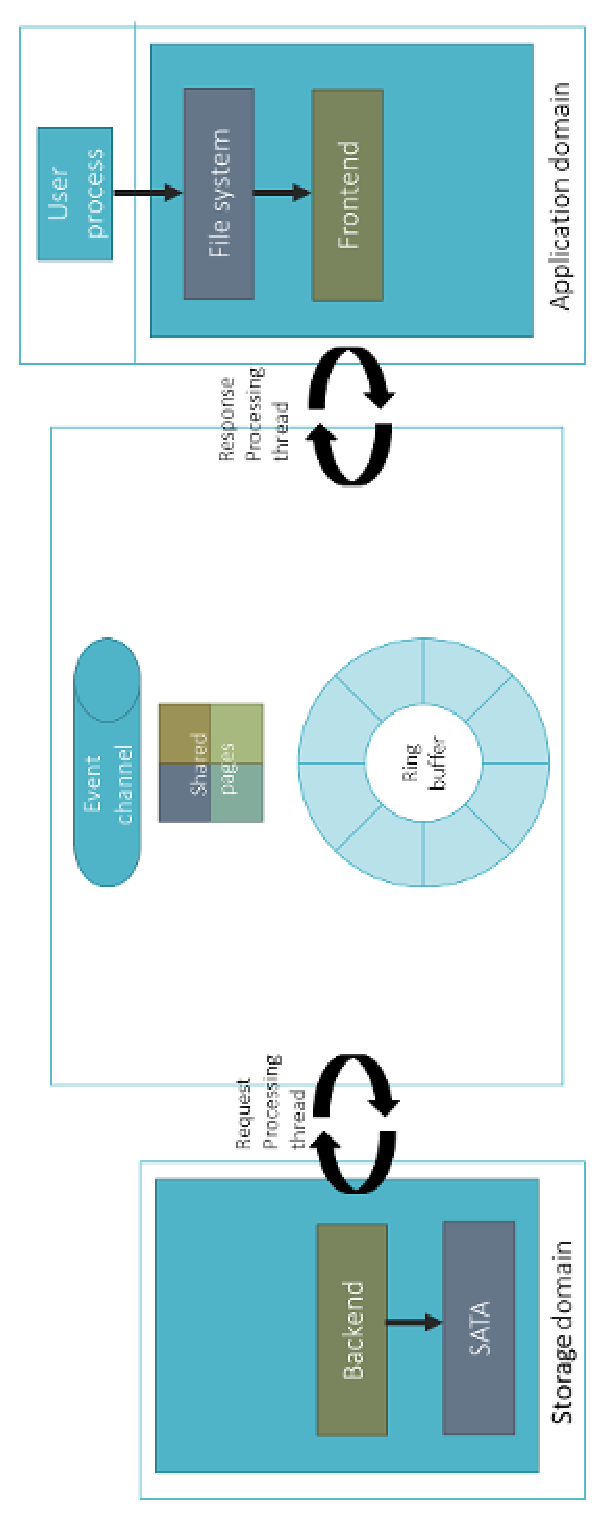
\includegraphics[scale=.5]{impl_overview}
\caption{Implementation overview}
\label{fig:Implementation overview}
\end{figure}

\subsection{Communication component}
The most important component in the Xen driver domain system implementation is the communication component. 
\\
This section will describe the implementation details of the communication channel of xen driver domain system and the implementation details to improve performance of the commmunication channel.
\begin{enumerate}
\item In the original implementation of the communication channel, event channel is used for notifying driver domain domU and application domain when a request or response is available in the shared request and response queue.  
\item In order to improve the performance of the system, we implement the communication channel in which the front end driver thread spins for the availablity of responses, and a dedicated thread in the back end driver spins for requests. In case of unavailablity of requests and responses, threads go to sleep. In this implementaion event channel is used only to wake these threads up from the remote domain.
\end{enumerate}

The following subsections describe the implementation details of the communication channel with and without performance improvement measures.

\subsubsection*{Ring buffer: I/O rings}
\label{subsec:ringbuf}
In the implementation of communication channel, for both approaches, ring buffer is used as a request and response queue. Ring buffer is a shared I/O ring explained in section~\ref{subsec:io rings}. A ring buffer is divided into front ring and back ring. The front ring is used as a request queue and  the back ring is used as a response queue. The front end driver recieves the request from an application, and converts the request into a format which  can be understood by the back end driver. The front end device driver then checks for a free space in the request queue for a new request, and allocates the space for the new request using the function \texttt{RING\_GET\_REQUEST}. 
\begin{verbatim}
ring_req = RING_GET_REQUEST(&info.main_ring, info.main_ring.req_prod_pvt);
if(ring_req == NULL){
 printk("NULL RING_GET_REQUEST\n");
 BUG_ON(1);
 return 1;
}
ring_req->seq_no = id;
ring_req->sector_number = blk_rq_pos(req);
ring_req->data_direction=write;
\end{verbatim}
After batching sufficient requests together, the front end device driver pushes the requests to the front ring using the function \texttt{RING\_PUSH\_REQUESTS\_AND\_CHECK\_NOTIFY}
\begin{verbatim}
static inline void flush_requests(idd_irq_info_t *flush_info)
{
 int notify;
 RING_PUSH_REQUESTS_AND_CHECK_NOTIFY(&flush_info->main_ring, notify);
 notify_remote_via_irq(flush_info->ring_irq);
}
\end{verbatim}

\subsubsection*{Shared pages}
Since the ring buffer is not large enough to hold the read and write data of responses and requests, we use it only for sharing the requests and responses. In order to share an actual data we use shared pages. 

\subsubsubsection*{Grant Table} 
Grant tables are a mechanism provided by the Xen hypervisor for sharing and transferring frames between the domains. It is an interface for granting foreign access to machine frames and sharing memory between underprivileged domains provided by the Xen hypervisor. In Xen, each domain has a respective grant table data structure, which is shared with the Xen hypervisor. The grant table data structure is used by Xen to verify the access permission other domains have on the page allocated by a domain\cite{granttable}.

\subsubsubsection*{Grant References}
Grant references are the entries in the grant table. A grant reference entry has every detail about the shared page, which removes the dependency on the real machine address of the shared page. Since there exists a fully virtualized memory, the biggest difficulty in sharing the memory correctly between domains is knowing its correct machine address. Removing the dependency with the real machine address makes it possible to share the memory between domains.\cite{Chisnall:2007:DGX:1407351, Barham:2003:XAV:945445.945462, granttable} 
\\
We use grant table so that the application domain grants the driver domain access to the the shared page, while retaining the ownershipn. The front end driver grants memory access to the back end driver, so that back end driver may read or write data into the shared memory as requested.
\\
The steps we implement are:
\begin{enumerate}
\item The application domain creates a grant access reference, and shares the reference id (ref) to the block device driver domain by enqueueing a request in the request queue (front I/O ring) .
\item The block device driver domain reads the request and the reference id, and uses the reference to map the foreign access granted frame.
\item The block device driver domain performs the memory access.
\item The block device driver domain unmaps the granted frame.
\item The application domain removes its grant.
\end{enumerate}

\begin{enumerate}
\item Granting foreign domain access
\begin{verbatim}
for_each_sg(info.sg, sg, ring_req->nr_segments, i) {
  buffer_mfn = pfn_to_mfn(page_to_pfn(sg_page(sg)));
  fsect = sg->offset >> KERNEL_SECTOR_SHIFT;
  lsect = fsect + (sg->length >> KERNEL_SECTOR_SHIFT) - 1;
   
  ref = gnttab_claim_grant_reference(&gref_head);
  BUG_ON(ref == -ENOSPC);
    
  gnttab_grant_foreign_access_ref(ref, info.domid,.
  buffer_mfn, rq_data_dir(req));

  info.shadow[id].frame[i] = mfn_to_pfn(buffer_mfn);
  ring_req->seg[i] = (struct idd_request_segment) {
      .gref       = ref,
      .first_sect = fsect,
      .last_sect  = lsect };
}
\end{verbatim}

\item Mapping foreign frames
\begin{verbatim}
for (i = 0; i < nseg; i++) { 
  flags = GNTMAP_host_map ;
  if (pending_req->operation != 0)
     flags |= GNTMAP_readonly;

  gnttab_set_map_op(&map[i], vaddr(pending_req, i),
  flags, req->seg[i].gref, DOMZERO);
}

ret = gnttab_map_refs(map, NULL, &backend.pending_page(pending_req, 0), nseg);
BUG_ON(ret);
 
for (i = 0; i < nseg; i++) {
  if (unlikely(map[i].status != 0)) {
    printk("invalid buffer -- could not remap it\n");
    map[i].handle = IDD_INVALID_HANDLE;
    ret |= 1;
  }

  pending_handle(pending_req, i) = map[i].handle;
  if(ret)
    continue; 
	seg[i].buf = map[i].dev_bus_addr |.
	(req->seg[i].first_sect << KERNEL_SECTOR_SHIFT);
}
\end{verbatim}

\item Unmapping foreign frames
\begin{verbatim}
for (i = 0; i < req->nr_pages; i++) {
	handle = pending_handle(req, i); 
  if(handle == IDD_INVALID_HANDLE)
    continue;
  gnttab_set_unmap_op(&unmap[invcount], vaddr(req, i), 
      GNTMAP_host_map, handle);
  pending_handle(req, i) = IDD_INVALID_HANDLE;
  pages[invcount] = virt_to_page(vaddr(req, i));
  invcount++;
}  
ret = gnttab_unmap_refs(unmap, pages, invcount, 0); 
\end{verbatim}

\item End foreign access
\begin{verbatim}
for (i = 0; i < s->req.nr_segments; i++) {
	gnttab_end_foreign_access(s->req.seg[i].gref, 0, 0UL);
}
\end{verbatim}
\end{enumerate}

\texttt{gnttab\_end\_foreign\_access} does not revoke access; it only prevents further mappings. Since \texttt{gnttab\_end\_foreign\_access} does not revoke access it is used after the block device driver has unmapped the frame\cite{Chisnall:2007:DGX:1407351, Barham:2003:XAV:945445.945462}.

%------------- proof read --
\subsubsection*{Event Channel}
Event channel is a mechanism provided by xen hypervisor for event notification. Xen Driver domain implementation use event channel to send notifications between domains that request and response is available in the request and response queue.
\\
However, in the implementation to improve the performance of the communication channel and hence the system we spin threads to share request and responses between domains and event channel is used only to wake up the both threads.

\subsubsubsection*{Event channel : Hypercall interface}

\texttt{EVTCHNOP\_alloc\_unbound} is a hypercall to allocate a new event channel port. Allocated event channel port can be connected by remote domain if,
\begin{enumerate}
\item Specied domain exist
\item A free port exist in the specified domain.
\end{enumerate}
Less privileged domains can allocate only their own ports, privileged domains can also allocate ports in other domains\cite{Chisnall:2007:DGX:1407351, Barham:2003:XAV:945445.945462}. 
\texttt{bind\_evtchn\_to\_irqhandler} is used for assigning an interrupt handler for a notification.
In driver domain implementation, back end driver allocates an event channel while initializing, and assigns an interrupt handler. 
\begin{verbatim}
ring_alloc.dom = DOMID_SELF;
ring_alloc.remote_dom = DOMZERO;
smp_mb();
err = HYPERVISOR_event_channel_op(EVTCHNOP_alloc_unbound, &ring_alloc);
if (unlikely(err != 0))
  goto end2;
\end{verbatim}

\subsubsubsection*{Event channel: Other interfaces}

\texttt{bind\_interdomain\_evtchn\_to\_irqhandler} is used for connecting to existing event channel as well as assigning an interrupt handler for handling a notification. In driver domain implementation back end driver allocates the event channel, and binds the interrupt handler to allocated event channel using \texttt{bind\_interdomain\_evtchn\_to\_irqhandler}.

\begin{verbatim}
err = bind_evtchn_to_irqhandler(ring_alloc.port, irq_ring_interrupt,
  0, "syscall_backend_irq_ring", &backend);
\end{verbatim}
In driver domain implementation, front end driver connects to the event channel allocated by backend, using interface \texttt{bind\_interdomain\_evtchn\_to\_irqhandler}.  
\begin{verbatim}
err = bind_interdomain_evtchn_to_irqhandler(data.domid, data.ring_port,
    irq_ring_interrupt, 0, "ring_irq", NULL);
if (unlikely(err < 0)) {
	printk(KERN_WARNING "Cannot bind (main) event channel\n");
	goto end2;
}
\end{verbatim}

\subsection{Application domain}
Application domain is the domain running user applications. In the monolithic linux kernel, usually an user process sends the read write request to file system, which sends the read and write request to the block device driver. The block device driver serves the request and send back a response to the file system, which further sends the response to the user process. 
\\ 
In Xen driver domain implementation block device runs separately in a driver domain. When user process sends a request to the file system, the file system needs to forward the request to storage domain. Like explained in the section~\ref{subsec:frontend}, in the implementation of xen driver domain, a piece of code is introduced which forwards the request to the domU running device drivers. 

\subsubsection*{Front end driver}

The piece of code, which forwards the request to the domU running device driver is called as a Front end driver. The core responsibility of the front end driver is:
\begin{enumerate}
\item To provide an interface which appears as a block device to upper layer in the stack.
\item Accept a request from the upper layer.
\item Create a new request which can be understood by storage domain.
\item Enqueue new request into request queue.
\end{enumerate}

Implementation details of front end driver is split into 4 stages. 
\begin{enumerate}
\item Initialization
\item Create request
\item Enqueue request 
\item Dequeue response
\end{enumerate}

\subsubsubsection*{Initialization}
During the initialization process the front end driver creates an interface for all the block devices. After creating the interface for all block devices, front end driver creates a kernel thread \texttt{read\_response\_thread}
\begin{verbatim}
info.response_thread = kthread_run(idd_read_response, &info, "read_response_thread");
\end{verbatim}
The core functionality of the \texttt{read\_response\_thread} is to dequeue the responses available in the ring buffer. However, there might be a case when no request is available in the ring buffer, but the request is expected to be present in the future. In such cases, \texttt{read\_response\_thread} thread spins for the responses.
\\
The \texttt{read\_response\_thread} thread goes into sleep state after spinning for some time- threshold. 
\\
Obviously, a thread shouldn't sleep unless it is assured that somebody else, somewhere, will wake it up. The code doing the waking up job must also be able to identify the thread to be able to do its job. We use a data structure called a wait queue to find the sleeping thread. A wait queue is a list of threads, all waiting for a specific event\cite{galvin, Bovet:2005:ULK:1077084}.
\\
In Linux kernel like all other lists, a wait queue is managed by a wait queue head, of a data type \texttt{wait\_queue\_head\_t}, and is defined in \texttt{$<linux/wait.h>$}. A wait queue head is defined and initialized statically as follows:
\texttt{DECLARE\_WAIT\_QUEUE\_HEAD(name);}
and dynamicly as follows:
\texttt{wait\_queue\_head\_t my\_queue;}
\texttt{init\_waitqueue\_head(\&my\_queue);}

\begin{verbatim}
info.response_thread = kthread_run(idd_read_response, &info, "read_response_thread");
init_waitqueue_head(&info.wq);
info.waiting_rsps=1;
\end{verbatim}

\subsubsubsection*{Create request}
Front end driver dequeues the request submitted to the driver interface by an user process or the file system, and then converts the request into a request of structure type \texttt{idd\_request\_t}. The structure is as below:

\begin{verbatim}
struct idd_request {
  int data_direction; 
  uint8_t nr_segments;
  uint64_t sector_number;
  struct idd_request_segment {
      grant_ref_t gref;
      uint8_t first_sect, last_sect;
  }seg[IDD_MAX_SEGMENTS_PER_REQUEST];
  uint64_t seq_no;
}__attribute__((__packed__));
\end{verbatim}

Member of the structure are explained below.
\texttt{data\_direction} : Flag to tag if request is read or write.
\texttt{nr\_segments} : Number of \texttt{idd\_request\_segment}s.
\texttt{gref} : Grant reference\/ grant table entry.
\texttt{first\_sect} and \texttt{last\_sect} : first and last sector in frame to transfer.
\texttt{seq\_no} : To track if any request and response is lost.

\subsubsubsection*{Enqueue request}

Like explained in section~\ref{subsec:ringbuf}, \texttt{RING\_PUSH\_REQUESTS\_AND\_CHECK\_NOTIFY} is used for flushing request to the ring buffer, we use the same API to enqueue the request to the request queue.
\begin{verbatim}
  RING_PUSH_REQUESTS_AND_CHECK_NOTIFY(&flush_info->main_ring, notify);
\end{verbatim}
However, if the \texttt{read\_request\_thread} running in back end driver which accepts the requests is sleeping, then waking up the \texttt{read\_request\_thread} is more important task of front end driver. Wake up signal is sent to back end driver using an event channel. Before sending the notification, we check the state of the thread.
\begin{verbatim}
status = atomic_read(&(flush_info->main_ring.sring->req_status));
smp_mb();

if(status == SLEEPING){
  notify_remote_via_irq(flush_info->ring_irq); 
\end{verbatim}
Status of the thread is saved in the shared memory. We use the atomic variables to save the state of threads to avoid race conditions. 

\subsubsubsection*{Dequeue response}

Response is dequeued from the ring buffer by the \texttt{read\_response\_thread}. To dequeue the response from response queue, we use the ring buffer API \texttt{RING\_GET\_RESPONSE}. However, the important part in this stage it managing the \texttt{read\_response\_thread} thread. 
\\
When the response is not available \texttt{read\_response\_thread} spins for some time, and then goes to sleep. When the response is made available by the backend then depending upon the state of the thread, event channel interrupt is sent by the backend. If \texttt{read\_response\_thread} is in sleeping state then the backend driver will send an interrupt and the front end driver will wake up the thread, otherwise, no action is taken as thread is already spinning for the response.
\\
In interrupt handler shared atomic variable status is read by the front end driver and depending upon state action is taken.
\begin{verbatim}
status = atomic_read(&(info.main_ring.sring->rsp_status));
if(status == SLEEPING){
  wake_up(&info.wq);
	info.waiting_rsps = 1;
}
atomic_set(&(info.main_ring.sring->rsp_status), RUNNING);
smp_wmb();
\end{verbatim}
\texttt{read\_response\_thread} sleeps on the wait queue \texttt{info.wq} waiting for \texttt{info.waiting\_rsps} to be set.
\\
\begin{verbatim}
wait_event_interruptible(
  info.wq,
  info.waiting_rsps || kthread_should_stop());
\end{verbatim}
Response is read using  ring buffer API \texttt{RING\_GET\_RESPONSE}.
\begin{verbatim}
rp = info.main_ring.sring->rsp_prod;

for (i = info.main_ring.rsp_cons; i != rp; i++) {
  unsigned long id;
  sleep_cond = 0;
  ring_rsp = RING_GET_RESPONSE(&info.main_ring, i);
  id  = ring_rsp->seq_no;
  if (id >= IDD_RING_SIZE)
    continue;
\end{verbatim}
We also maintain an shadow table of all requests which are ended upon reading respective successful response. 
\begin{verbatim}
  req  = info.shadow[id].request;
  if(req!=NULL)
    idd_completion(&info.shadow[id], ring_rsp);
  if (add_id_to_freelist(&info, id)) {
    WARN(1, "response to %s (id %ld) couldn't be recycled!\n",
      op_name(ring_rsp->op), id);
    continue;
  }
  error = (ring_rsp->res == 0) ? 0 : -EIO;
  __blk_end_request_all(req, 0);
}
\end{verbatim}
Upon reading the responses, thread spins again for more responses and then goes to sleep.    
We mark the state of the thread as \texttt{SLEEPING} and then check for the request queue to avoid race condition. If a request is present in the request queue then the request is served while state of the thread is still \texttt{SLEEPING}.
\begin{verbatim}
status = atomic_read(&(info.main_ring.sring->rsp_status));
if(sleep_cond > THRESHOLD && status==RUNNING){
  atomic_set(&(info.main_ring.sring->rsp_status), SLEEPING);
  info.waiting_rsps = 0;
  sleep_cond = 0;
  RING_FINAL_CHECK_FOR_RESPONSES(&info.main_ring, more_to_do);
  if (more_to_do)
    goto again;
}
\end{verbatim}

\subsection{Driver domain}

Driver domain is the domU running a device driver. In our implementation, driver domain runs block device driver. Usually in monolithic linux kernel an user process sends the read write request to a file system, which sends the read and write request to block device driver. Block device driver serves the request and responses back to file system, which further sends response to user process.
\\  
However, in driver domain implementation, block device runs separately in a driver domain. Like explained in a section~\ref{subsec:backend}, a peice of code called as a back end driver runs in a driver domain which accepts a request from application domain and forward the request to the device driver. Upon receiving the reponse from the device driver, back end driver sends back the response, and notifies the application domain.

\subsubsection*{Back end driver}

Back end driver is a kernel module and component of independent block device driver which runs in the storage domain. The core responsibility of back end end driver is :
\begin{enumerate}
\item Dequeue resquest from request queue.
\item Convert to BIO request which can be understood by block device driver .
\item Accept response from block device driver.
\item Enqueue response into response queue.
\end{enumerate}
Implementation details of back end driver can be split into 5 stages. 
\begin{enumerate}
\item Initialization
\item Dequeue request
\item Create BIO. 
\item Make response.
\item Enqueue response
\end{enumerate}

\subsubsubsection*{Initialization}
During initialization process Back end driver creates a kernel thread \texttt{read\_request\_thread}.
\begin{verbatim}
backend.request_thread = kthread_run(idd_request_schedule, &backend, "read_request_thread");
\end{verbatim}

The core functionality of the \texttt{read\_request\_thread} is to dequeue the requests available in the request queue. If request is not available in the request queue then thread waits on a wait queue. Similar to front end, back end driver initializes wait queue in initiazation process. 

\subsubsubsection*{Dequeue request}
Request is dequeued from the request queue by the \texttt{read\_resquest\_thread}. To dequeue a request, we use the ring buffer API \texttt{RING\_GET\_RESPONSE}. When the request queue is empty, \texttt{read\_resquest\_thread} spins for some time to checks if new requests are queued, after reaching threshold it goes to sleep. When the request is enqueued by front end driver then depending upon the state of the \texttt{read\_resquest\_thread}, an event channel interrupt is sent by the front end driver. If \texttt{read\_resquest\_thread} is in a sleeping state then front end driver will send an interrupt. In intrupt handler, back end driver will wake up the \texttt{read\_resquest\_thread}. If \texttt{read\_resquest\_thread} is already running then no action is taken. In interrupt handler, status is read from shared atomic variable by the back end driver.

\begin{verbatim}
status = atomic_read(&(backend.main_ring.sring->req_status));
if(status == SLEEPING){
	wake_up(&backend.wq);
	backend.waiting_reqs = 1;
}
atomic_set(&(backend.main_ring.sring->req_status), RUNNING);
\end{verbatim}
\texttt{read\_resquest\_thread} sleeps on the wait queue \texttt{backend.wq} waiting for \texttt{backend.waiting\_reqs} to be set.
\begin{verbatim}
wait_event_interruptible(
	be->wq,
	be->waiting_reqs || kthread_should_stop());
\end{verbatim}
Request is read using ring buffer API \texttt{RING\_GET\_REQUESTS}.
\begin{verbatim}
rc = be->main_ring.req_cons;
rp = be->main_ring.sring->req_prod;
rmb();
while (rc != rp) {
  if (RING_REQUEST_CONS_OVERFLOW(&be->main_ring, rc))
    break;
  memcpy(&req, RING_GET_REQUEST(&be->main_ring, rc), sizeof(req));
  be->main_ring.req_cons = ++rc;
\end{verbatim}
Upon reading requests, thread spins again for more responses. If a threshold is reached then the thread goes to sleep. We mark the state of the thread as \texttt{SLEEPING} and then check for the request queue one more time to avoid a race condition. If request is present in request queue then that request is served while state of the thread is still \texttt{SLEEPING}.

\begin{verbatim}
status = atomic_read(&(backend.main_ring.sring->req_status));
if(sleep_cond > THRESHOLD && status==RUNNING){
  atomic_set(&(backend.main_ring.sring->req_status), SLEEPING);
  be->waiting_reqs = 0;
  sleep_cond=0;
  RING_FINAL_CHECK_FOR_REQUESTS(&be->main_ring, more_to_do);
  if (more_to_do)
    goto again;
\end{verbatim}

\subsubsubsection*{Create BIO}
\label{subsec:createbio}
Whenever the request thread receives a request to serve, the request thread creates the \texttt{bio} request for the corresponding request. \texttt{bio} structure is a basic container for block I/O within a kernel. \texttt{bio} structure is defined in \texttt{$<linux/blk_types.h>$}. \texttt{bio} structure represents active block I/O operations as a list of segments, and a segment is a chunk of buffers. The \texttt{bio} structure provides the capability for the kernel to perform block I/O operations of even a single buffer from multiple locations in memory. Vector I/O such as this is called scatter-gather I/O.
\\
Following is the struct bio:
\begin{verbatim}
struct bio {
  sector_t    bi_sector;  /* device address in 512 byte sectors */
  struct bio    *bi_next; /* request queue link */
  struct block_device *bi_bdev; /* associated block device */
  unsigned long   bi_flags; /* status, command, etc */
  unsigned long   bi_rw;    /* bottom bits READ/WRITE, top bits priority */
  unsigned short  bi_vcnt;  /* how many bio_vec's */
  unsigned short  bi_idx;   /* current index into bvl_vec */
  unsigned int    bi_phys_segments; /* Number of segments in this BIO after physical address coalescing is performed. */
  unsigned int    bi_size;  /* residual I/O count */
  unsigned int    bi_seg_front_size;
  unsigned int    bi_seg_back_size;
  unsigned int    bi_max_vecs;  /* max bvl_vecs we can hold */
  atomic_t    bi_cnt;   /* pin count */
  struct bio_vec    *bi_io_vec; /* the actual vec list */
  bio_end_io_t    *bi_end_io;  void      *bi_private;
  bio_destructor_t  *bi_destructor; /* destructor */
  struct bio_vec    bi_inline_vecs[0];
};
\end{verbatim}
A request queued into the request queue by the front end driver is in format which is understood by back end driver, but we can not forward the same request to block device. We convert the dequeued request into \texttt{bio} request, so that the block device understands the request. To make the \texttt{bio} request, we need the associated block device structure \texttt{struct block\_device}. We get associated block device structure using function \texttt{blkdev\_get\_by\_path}.
\begin{verbatim}
backend.bdev = blkdev_get_by_path("/dev/ramd",
  FMODE_READ | FMODE_WRITE | FMODE_LSEEK |
  FMODE_PREAD | FMODE_PWRITE, NULL);

backend.dev = MKDEV(MAJOR(backend.bdev->bd_inode->i_rdev),
  MINOR(backend.bdev->bd_inode->i_rdev));
\end{verbatim}
Pages from shared memory are mapped and inserted into the \texttt{bio} structure using function \texttt{bio\_add\_page}. And other variables are copied into the \texttt{bio} structure from the dequeued request. 
\begin{verbatim}
for (i = 0; i < nseg; i++) {
  while ((bio == NULL) || bio_add_page(bio,
  be->pending_page(pending_req, i),
  seg[i].nsec << 9,.
  seg[i].buf & ~PAGE_MASK) == 0) {
    bio = bio_alloc(GFP_KERNEL, nseg - i );
    if (unlikely(bio == NULL))
      goto fail_put_bio;
    biolist[nbio++] = bio;  
    bio->bi_bdev = breq.bdev;
    bio->bi_private = pending_req;
    bio->bi_end_io = end_block_io_op;
    bio->bi_sector  = breq.sector_number;
  }
  breq.sector_number += seg[i].nsec;
}
\end{verbatim}
At the end, the newly created \texttt{bio} request is sent to the lower layer for execution. 
\begin{verbatim}
for (i = 0; i < nbio; i++){
  submit_bio(op, biolist[i]);
}
\end{verbatim}
\texttt{bi\_end\_io} function pointer is a pointer to a callback function. Once bio request is completed, function pointed by \texttt{bi\_end\_io} gets called.
\begin{verbatim}
bio->bi_end_io = end_block_io_op; 
\end{verbatim}

\subsubsubsection*{Make response and Enqueue}
Irrespective of the success or failure of the execution of \texttt{bio} request, the back end driver makes a response, which could be understood by the frontend. Like explained in subsection~\ref{subsec:createbio}, \texttt{bi\_end\_io} function pointer is a pointer to a callback function. Once bio request is completed, function pointed by \texttt{bi\_end\_io} gets called. We create a new response in this callback function.
\\
In this callback function we complete the \texttt{bio} request with function \texttt{bio\_put}. After that the result gets copied into a newly allocated response structure. The response is enqueued to response queue using \texttt{RING\_GET\_RESPONSE} and \texttt{RING\_PUSH\_RESPONSES\_AND\_CHECK\_NOTIFY}. Once the response is enqueued, depending upon the status of the remote thread-\texttt{read\_response\_thread}, a inturrupt signal is sent to the application domain.
\begin{verbatim}
resp.op = op;
resp.seq_no = id;
resp.priv_data = NULL;
resp.res = st;
spin_lock_irqsave(&be->blk_ring_lock, flags);
memcpy(RING_GET_RESPONSE(&be->main_ring, backend.main_ring.rsp_prod_pvt),&resp, sizeof(resp));
be->main_ring.rsp_prod_pvt++;
RING_PUSH_RESPONSES_AND_CHECK_NOTIFY(&be->main_ring, notify);
status = atomic_read(&(be->main_ring.sring->rsp_status));
smp_mb();
if(status == SLEEPING){
  notify_remote_via_irq(be->ring_irq);
\end{verbatim}    

\pagebreak

% \bibliography{references}
\ifbool{toShowBibliography}{\bibliography{references}}{}

\chapter{Related Work}
\markright{Sushrut Shirole \hfill Chapter 5. Related Work \hfill}

% VirtuOS~\cite{Nikolaev:2013:VOS:2517349.2522719} is a library level solution that allows processes to directly communicate with domain. 

This chapter briefly discusses about the work closely related to the IDDR System. Since our work is divided into two parts: 1. Implementation of the Driver Domain to improve the robustness of the system 2. Performance improvement of the inter-domain communication, this chapter is divided into two section. Section~\ref{robustness} discusses the work which improves the robustness of the system and Section~\ref{interdomain} discusses the different work which concentrates on improving the inter-domain communication.
% \\[3mm]

% \section{Robustness of The System}

% \subsection{Driver Protection Approches}

% Because most kernel failures are caused by faulty device drivers, there is a particular focus on making them safer and isolating them from other system components. 

% 1 Nooks - introduced
% hardware protection domains inside a monolithic kernel to isolate device drivers from each
% other and from the remaining kernel. Such isolation protects against buggy drivers that
% may perform illegal memory accesses. Nooks demonstrated how to restructure an existing
% kernel’s interaction with its drivers to facilitate the use of intrakernel protection domains,
% and explored the trade-off between benefits due to isolation and costs imposed by the domain
% crossings this approach requires. This approach requires drivers to be adapted to the new
% mechanism, as their interaction with the OS kernel changes. Switching to and from protection domains requires page table switches, along with corresponding TLB flushes, which if done
% frequently may affect the performance of some applications

% 2. Microdrivers - 
% 3. SUD 

% split drivers into parts running inside the kernel and parts running as
% user processes. In microdrivers, hardware-specific and performance critical code remains in
% the kernel whereas the remaining code is moved to user space to provide better isolation.
% Additionally, code running in user space can be written in a higher-level language [80].
% Mainstream OS have provided support for writing device drivers that execute in user mode
% for some time, but these facilities have not been widely used because the added context
% switches made it difficult to achieve good performance [63]. Some systems provide the
% ability to run unchanged kernel components such as out-of-box Linux drivers in user mode.
% DD/OS [64] provides this ability by creating a virtual machine built as a user-level task
% running on top of L4, whereas SUD [21] provides such an environment inside ordinary Linux
% user processes. Xen Driver Domains [85] use a mechanism with comparable protection
% properties by running unchanged drivers in specialized guest OS. The Qubes OS [8] adopted
% the Xen hypervisor and Xen Driver Domains to enhance security by running separate virtual
% machines for drivers and applications. The Qubes OS supports a storage domain, a network
% domain and application virtual machine

% \subsubsection*{Virtualization Based Approches}

% Xen driver domain : 

% La vasseur - 


% \subsection*{Other Approches}
% 1. kernel based  :

% Microkernel Mach - A new kernel foundation for UNIX development
% Microkernel L4 - On micro-kernel construction 
% Both, architecture in which only essential functionality such as task scheduling and message-based interprocess communication is implemented inside the kernel, whereas most other system components, including device drivers, are implemented in separate user processes.


% Microvisors : Recently, microkernels have been used in lieu of hypervisors. Microvisors expose abstractions typical to hypervisors such as VCPUs, memory address space containers, and communication channels to run virtual machines with guest OS on top of a microkernel. [The OKL4 Microvisor: Convergence Point of Microkernels and Hypervisors]


% Dune uses hardware-assisted VMs to isolate applications from each other. Nested paging allows applications to switch their page tables efficiently. Process context switches benefit from TLB tagging available for hardware-assisted VMs. Dune also improves signal delivery latencies by delivering hardware interrupts directly to user processes. However, Dune still uses a monolithic kernel which does not isolate device drivers from each other. Additionally, applications may have to use more expensive hypercalls in lieu of system calls to access OS services. [Dune: Safe User-level Access to Privileged CPU Features.]




% \section{Inter-domain Communication}
% In the past numerous  work on inter domain communication mechanisms was presented. Xen split drivers is one of the inter domain communication approach of Xen hypervisor~\cite{Fraser04safehardware}. The xen split drivers has overhead becuase of numerous context switches in form of event channel interrupts. It also incurs an overhead due to data copy, page flipping~\cite{Zhang:2007:XHI:1516124.1516138}. Xen hypervisor also provides a UNIX domain socket like interface for high throughput interdomain communication on the same system called XenSocket~\cite{Zhang:2007:XHI:1516124.1516138}. XenSocket replaces the page flipping design of the split driver. However, XenSocket needs an existing socket interface APIs to be changed. 
% \\[3mm]
% Fido~\cite{Burtsev:2009:FFI:1855807.1855832} is a shared memory based inter domain communication mechanism. Fido implements the fast interdomain communication mechanism by reducing data copies in Xen hypervisor. In contrast our system improves the inter domain communication mechanism of Split device drivers by avoiding the context switches.
% \\[3mm]

% The Fido system [25] optimizes Xen’s interdomain communication facilities
% by allowing read-only data mappings to enable zero-copy communication. Fido amortizes
% costs but users need to sacrifice some security and protections guarantees.
\ifbool{toShowBibliography}{\bibliography{references}}{}


\chapter{Evaluation}
\markright{Sushrut Shirole \hfill Chapter 6. Evaluation \hfill}

We use Linux Kernel version 3.5.0 for both application domain and driver
domains. We use the Arch Linux distribution for the \texttt{x86\_64}
platform for our testing and performance evaluation. The specifications of
the system used for the evaluation are presented in Table~\ref{tab:config}.

\begin{table}
\caption{Hardware specifications}
\begin{center}
\begin{tabular}{ll}
  \hline
  \label{tab:config}
  System Parameter & Configuration \\
  \hline
  Processor & 2 X Quad-core AMD Opteron(tm) Processor 2380, 2.49 Ghz \\
  Number of cores & 4 per processor \\
  Hyperthreading & OFF \\
  L1 L2 cache & 64K/512K per core \\
  L3 cache & 6144K \\
  Main memory & 16Gb \\
  Storage & SATA, HDD 7200RPM \\
  \hline 
\end{tabular}
\end{center}
\end{table}

\section{Goals}
\label{sec:goals}
The goals of our evaluation are:
\begin{enumerate}
\item \textbf{Comparison  of Xen's isolated driver domain mechanism with the interrupt-based IDDR system:}

In order to verify that the interrupt-based IDDR system constitutes a suitable baseline against 
which to compare the spinning-based IDDR system, we compared our interrupt-based implementation
against Xen's isolated driver domain.  However, since the source code
of the isolated driver domain implementation is not available, we achieve this evaluation goal 
by comparing the performance of the interrupt-based IDDR system with Xen's regular
drivers, which use the same split device driver model.

\item \textbf{Performance impact of spinning-based optimizations:}

The second goal of the evaluation is to prove that the spinning-based implementation of the 
communication channel improves the performance of the interdomain communication and hence the IDDR system.

We achieve this evaluation goal by comparing the performance of the interrupt-based IDDR system 
with the spinning-based IDDR system.
\end{enumerate}

\section{Methodology}
\label{sec:methodology}
In order to measure the performance of the system, we run performance
tests using a variety of block devices. In order to cover a variety of
devices we use block devices such as SATA disks, ramdisks and loop
devices for the performance testing. A loop device is a device that provides 
a block device that is backed by a file.  A ramdisk is a block of a memory
that acts as a disk drive.

In order to conduct the performance tests, we format the block
device with the ext2 file system, and run the SysBench
benchmark~\cite{sysbench} on it. SysBench is a multi-threaded benchmark
tool for evaluating operating system performance. It includes different test
modes, one of which is FileIO.  The FileIO mode can be used to produce
different file I/O workloads. It runs a specified number of threads to
execute requests in parallel. We run the SysBench benchmark in FileIO
test mode to generate 128 files with \texttt{1GB} of total data. We
execute random reads, random writes, and a mix of random reads and writes
on all three devices. We set the block size to \texttt{16KB}. We vary
the number of SysBench threads from 1 to 32 to measure the throughput of
the system under different levels of concurrent access.

\section{Xen Split Device Driver vs Interrupt-based IDDR System}
As per our first evaluation goal discussed in Section~\ref{sec:goals},
we compare the interrupt-based IDDR system with Xen's split device driver.

\subsection*{Experimental Setup}

\subsubsection*{Xen Split Device Driver}
We create a ramdisk in domain 0. The guest domain (domain U) is configured
to access domain 0's ramdisk via a split device driver. 
We use the same setup for the loop device and the SATA disk. 
We format and mount the disk into a partition in the
guest domain using the ext2 file system in all cases. The SysBench 
benchmark is run on the mounted partitions as explained in 
Section~\ref{sec:methodology}.

\subsubsection*{Interrupt-based IDDR System}
In the Xen hypervisor, the domain 0 always runs as a paravirtualized guest (PV),
but domain U can be using both a hardware-assisted virtualization configuration (HVM) 
or a paravirtualized configuration.  In our setup we run domain U always
in HVM mode because HVM guests exhibit less system call overhead
and faster memory bandwidth compared to PV guests, as we observed
by running the system call micro-benchmark tool lmbench\cite{lmbench}. 

When comparing to Xen's split device drivers, the backend device driver executes
in domain 0 and the frontend device driver in domain U.  
To eliminate any performance differences that may be solely due the mode
of virtualization used, we matched the modes of virtualization
by running IDDR's backend and frontend drivers also in 
domain 0 and U, respectively.

\subsubsection*{Comparison}
We compare the throughput of Xen's split device driver and the
interrupt-based IDDR system in Figure~\ref{fig:iddrvsxen-ramdisk-rdwr}
and Figure~\ref{fig:iddrvsxen-loop-rd}. 
Figure~\ref{fig:iddrvsxen-ramdisk-rdwr} presents the
throughput of both systems when data is randomly read from a ramdisk and
written to it. Figure~\ref{fig:iddrvsxen-loop-rd} presents the throughput
when data is randomly read from a loop device.

On a loop device, the performance of the interrupt-based IDDR system
differs by 3\%-4\% when compared to Xen's split device driver. On a
ramdisk, the throughput of the interrupt-based IDDR system matches that
of the Xen split device driver. This shows that our interrupt-based
IDDR implementation provides a suitable baseline for our performance 
optimizations.

\begin{figure}[!ht]
\centering
  \begin{subfigure}[b]{\textwidth}
  \includegraphics[width=\textwidth]{iddrvsxen-ramdisk-rdwr}
  \caption{Random reads and writes on a ramdisk}
  \label{fig:iddrvsxen-ramdisk-rdwr}
  \end{subfigure}\\
  \begin{subfigure}[b]{\textwidth}
  \includegraphics[width=\textwidth]{iddrvsxen-loop-rd}
  \caption{Random reads on a loop device}
  \label{fig:iddrvsxen-loop-rd}
  \end{subfigure}
\end{figure}

\begin{figure}[H]
  \ContinuedFloat
  \begin{subfigure}[b]{\textwidth}
  \includegraphics[width=\textwidth]{iddvsxen-harddisk-rd}
  \caption{Random reads on a SATA disk}
  \label{fig:iddrvsxen-harddisk-rd}
  \end{subfigure}\\
\caption{Interrupt-based IDDR system vs Xen split driver}\label{fig:seqloopdisk}
\end{figure}

\section{Interrupt-based IDDR System vs Spinning-based IDDR System}
We measure and compare the performance of the interrupt-based IDDR system
with the spinning-based IDDR system. To compare the performance of both
systems, we measure performance of the system by varying the number of
SysBench threads. The SysBench benchmark executes random reads and writes 
on a ramdisk, loop device, and a SATA disk.

\subsection*{Experimental Setup}
In both systems, the application domain is domain 0, and the driver domain
is domain U.  We create a ramdisk and insert the backend driver in the
driver domain.  We insert the frontend driver in the application domain.
We measure the performance of both systems on a loop device with the
same setup.

However, we were unable to set up PCI passthrough for the SATA disk,
preventing us from running the SATA controller driver in domain U.
For the SATA portion of the experiments, we use domain 0 as the
driver domain and domain U as the application domain, while still
retaining all other aspects of the IDDR implementation.

\subsubsection*{Random reads and writes}

\paragraph{Comparison:}

Figure~\ref{fig:rndramdisk}, Figure~\ref{fig:rndloopdisk}, and
Figure~\ref{fig:rndharddisk} compare the throughput of the interrupt-based
IDDR and the spinning-based IDDR system for read, write, and read/write
workloads using a ramdisk, loop device, and SATA disk, respectively.

Figure~\ref{subfig:rndrd-ramdisk}, Figure~\ref{subfig:rndrd-loopdisk},
and Figure~\ref{subfig:rndrd-harddisk} show that the spinning-based IDDR
system performs better when data is read from a device randomly.

Figure~\ref{subfig:rndwr-ramdisk}, Figure~\ref{subfig:rndwr-loopdisk}
and Figure~\ref{subfig:rndwr-harddisk} compare the performance of
the device when data is written randomly to a device. The graph shows
that initially the spinning-based IDDR system performs better than the
interrupt-based IDDR system, but as the number of SysBench threads increases,
the throughput of the spinning-based IDDR system decreases.

Figure~\ref{subfig:rndrw-ramdisk}, Figure~\ref{subfig:rndrw-loopdisk}
and Figure~\ref{subfig:rndrw-harddisk} compare the performance for mixed
random read and write workloads.

\begin{figure}[!ht]
 \centering
  \begin{subfigure}[b]{\textwidth}
  \includegraphics[width=\textwidth]{rndrd-ramdisk}
  \caption{Random reads}
  \label{subfig:rndrd-ramdisk}
  \end{subfigure}\\
  \begin{subfigure}[b]{\textwidth}
  \includegraphics[width=\textwidth]{rndwr-ramdisk}
  \caption{Random writes}
  \label{subfig:rndwr-ramdisk}
  \end{subfigure}
\end{figure}

\begin{figure}[H]
  \ContinuedFloat
  \begin{subfigure}[b]{\textwidth}
  \includegraphics[width=\textwidth]{rndrw-ramdisk}
  \caption{Random reads writes}
  \label{subfig:rndrw-ramdisk}
  \end{subfigure}
  \caption{Random reads and writes on a ramdisk}\label{fig:rndramdisk}
\end{figure}

\begin{figure}[!ht]
\centering
  \begin{subfigure}[b]{\textwidth}
  \includegraphics[width=\textwidth]{rndrd-loopdisk}
  \caption{Random reads}
  \label{subfig:rndrd-loopdisk}
  \end{subfigure}\\
  \begin{subfigure}[b]{\textwidth}
  \includegraphics[width=\textwidth]{rndwr-loopdisk}
  \caption{Random writes}
  \label{subfig:rndwr-loopdisk}
  \end{subfigure}
\end{figure}

\begin{figure}[H]
  \ContinuedFloat
  \begin{subfigure}[b]{\textwidth}
  \includegraphics[width=\textwidth]{rndrw-loopdisk}
  \caption{Random reads writes}
  \label{subfig:rndrw-loopdisk}
  \end{subfigure}
\caption{Random reads and writes on a loop device}\label{fig:rndloopdisk}
\end{figure}

\begin{figure}[!ht]
\centering
  \begin{subfigure}[b]{\textwidth}
  \includegraphics[width=\textwidth]{rndrd-harddisk}
  \caption{Random reads}
  \label{subfig:rndrd-harddisk}
  \end{subfigure}\\
  \begin{subfigure}[b]{\textwidth}
  \includegraphics[width=\textwidth]{rndwr-harddisk}
  \caption{Random writes}
  \label{subfig:rndwr-harddisk}
  \end{subfigure}
\end{figure}

\begin{figure}[H]
  \ContinuedFloat
  \begin{subfigure}[b]{\textwidth}
  \includegraphics[width=\textwidth]{rndrw-harddisk}
  \caption{Random reads writes}
  \label{subfig:rndrw-harddisk}
  \end{subfigure}
\caption{Random reads and writes on a SATA disk}\label{fig:rndharddisk}
\end{figure}

\paragraph{Observation:}
The performance analysis of the interrupt-based and spinning-based IDDR system
shows that initially the throughput of both systems increases and then it
remains constant. We measure the throughput of the system with varying
number of SysBench threads.

In both systems, when the number of SysBench threads is low,
the rate at which data is read and written is low and when the number of
SysBench threads is high, the rate at which data is read and written is
high.  Once maximum throughput is achieved, it remains constant.

In the interrupt-based IDDR system, virtual interrupts are sent between
application and driver domains whereas the spinning-based approach
attempts to avoid these virtual interrupts.  
Our optimization technique reduces the frequency of the
virtual interrupt being sent between domains. 
The higher performance gains at lower levels of concurrency
may be due to missed opportunities for batching in the interrupt-based case,
increasing the need for virtual interrupts even further.

\subsubsection*{CPU utilization}

The spinning-based IDDR system uses CPU cycles that could also be
used by applications unless excess CPU capacity is available (as in many
multicore or manycore systems). Hence we exploit a trade-off between higher 
CPU utilization and higher throughput.

In this section we compare the CPU utilization of the interrupt-based and
the spinning-based IDDR systems. Figure~\ref{fig:cpuramdisk}, Figure~\ref{fig:cpuloopdisk}, and
Figure~\ref{fig:cpuharddisk} compare the CPU utilization of both 
systems using the ramdisk, loop device and SATA disk setups.

\paragraph{Observation: }
In the spinning-based version of IDDR, the read response and request threads
spin continuously unless the driver is idle for extended periods of time.
Thus, up to 2 cores of the system may be consumed just for spinning.
Figures~\ref{fig:cpuramdisk} and~\ref{fig:cpuloopdisk} show the CPU
utilization for the ramdisk and loop device setups.
It can be seen that the CPU utilization of the spinning-based 
implementation ranges between 100\% and 250\%, which is within the
expected range.

\begin{figure}[!ht]
\centering
  \begin{subfigure}[b]{\textwidth}
  \includegraphics[width=\textwidth]{cpu-rndrd-ramdisk}
  \caption{Random reads}
  \label{subfig:cpu-rndrd-ramdisk}
  \end{subfigure}\\
  \begin{subfigure}[b]{\textwidth}
  \includegraphics[width=\textwidth]{cpu-rndrw-ramdisk}
  \caption{Random writes}
  \label{subfig:cpu-rndrw-ramdisk}
  \end{subfigure}
\end{figure}

\begin{figure}[H]
  \ContinuedFloat
  \begin{subfigure}[b]{\textwidth}
  \includegraphics[width=\textwidth]{cpu-rndwr-ramdisk}
  \caption{Random reads writes}
  \label{subfig:cpu-rndwr-ramdisk}
  \end{subfigure}
\caption{Comparison of CPU utilization - ramdisk}\label{fig:cpuramdisk}
\end{figure}

\begin{figure}[!ht]
  \begin{subfigure}[b]{\textwidth}
  \includegraphics[width=\textwidth]{cpu-rndrd-loopdisk}
  \caption{Random reads}
  \label{subfig:cpu-rndrd-loopdisk}
  \end{subfigure}\\
  \begin{subfigure}[b]{\textwidth}
  \includegraphics[width=\textwidth]{cpu-rndrw-loopdisk}
  \caption{Random writes}
  \label{subfig:cpu-rndrw-loopdisk}
\end{subfigure}
\end{figure}

\begin{figure}[H]
  \ContinuedFloat  \begin{subfigure}[b]{\textwidth}
  \includegraphics[width=\textwidth]{cpu-rndwr-loopdisk}
  \caption{Random reads writes}
  \label{subfig:cpu-rndwr-loopdisk}
  \end{subfigure}
\caption{Comparison of CPU utilization - loop device}\label{fig:cpuloopdisk}
\end{figure}

\begin{figure}[!ht]
\centering
  \begin{subfigure}[b]{\textwidth}
  \includegraphics[width=\textwidth]{cpu-rndrd-harddisk}
  \caption{Random reads}
  \label{subfig:cpu-rndrd-harddisk}
  \end{subfigure}\\
  \begin{subfigure}[b]{\textwidth}
  \includegraphics[width=\textwidth]{cpu-rndwr-harddisk}
  \caption{Random writes}
  \label{subfig:cpu-rndwr-harddisk}
  \end{subfigure}
\end{figure}

\begin{figure}[H]
  \ContinuedFloat
  \begin{subfigure}[b]{\textwidth}
  \includegraphics[width=\textwidth]{cpu-rndrw-harddisk}
  \caption{Random reads writes}
  \label{subfig:cpurndrw-harddisk}
  \end{subfigure}
\caption{Comparison of CPU utilization - SATA disk}\label{fig:cpuharddisk}
\end{figure}

\chapter{Conclusion and Future Work}
\markright{Sushrut Shirole \hfill Chapter 7. Conclusion and Future Work \hfill}

In this thesis we presented the Isolated Device Driver (IDDR) system. The IDDR system is an operating system which provides isolation between a device driver and the Linux kernel components by running the device driver in the driver domain. The IDDR system is a re-implementation of the Xen's isolated driver domain.
\\[3mm]
In Xen's isolated driver domain, a domain communicates with a device driver running in the priviledged domain through a split device driver mechanism. The split device driver follows an interrupt based approach. We replaced the interrupt based approach with the spinlock based approach. The spinlock based approach avoids the unwanted domain rescheduling for every software interrupt. The IDDR system trades of CPU cycles for the benefit of the performance.
\\[3mm]
We tested the IDDR system with different block devices, and the experimental evaluation has shown that the IDDR system performs better by compromizing the CPU utilization. 
\\[3mm]
The IDDR system will be advantagious if used with I/O intensive applications. In the I/O intesive applications, when the workload is low, the CPU utilization is also low. Hence the IDDR system can afford to waste the idle CPU cycles for the benefit of the performance. On the other hand, in case of heavy workload, the CPU utilization is high. Hence if the IDDR system utilizes the CPU cycles in order to improve the performance, it is still acceptable, as those CPU cycles would have been used anyway. However, the IDDR system will hinder the performance of the system, if the system is running CPU intensive applications with an average IO workload.


%%%%%%%%%%%%%%%%
% Do tables like this:

%  \begin{table}
%  \caption{The Graduate School wants captions above the tables.}
% \begin{center}
%  \begin{tabular}{ccc}
%  x & 1 & 2 \\ \hline
%  1 & 1 & 2 \\
%  2 & 2 & 4 \\ \hline
%  \end{tabular}
% \end{center}
%  \end{table}

%%%%%%%%%%%%%%%%%
% all sections and sub-sections

%\part
%\chapter (report style only)
%\section
%\subsection
%\subsubsection
%\paragraph
%\subparagraph
%\subsubparagraph (milstd and book-form styles only)
%\subsubsubparagraph (milstd and book-form styles only)

%%%%%%%%%%%%%%%%%%%%%%%%%%%%%%%%

%\chapter*{Bibliography}
\nocite{*}
\bibliographystyle{plain}
\bibliography{references}

% \appendix

% In LaTeX, each appendix is a "chapter"
% \chapter{Program Source}

\end{document}


%
%


